\subsection*{Wybór modeli}
Porównano trzy sieci konwolucyjne (kod: \texttt{src/models.py}):
\begin{enumerate}
\item \textbf{CNN uczona od zera} (\cvParamsCnn{} mln parametrów): 4 bloki
  [Conv 3$\times$3 -- BatchNorm -- ReLU]$\times$2 + MaxPool (32--256 filtrów), globalne
  uśrednianie, dropout i warstwa liniowa. Punkt odniesienia, który pokazuje, ile daje
  transfer wiedzy.
\item \textbf{EfficientNetB0} (\cvParamsEff{} mln parametrów) z wagami ImageNet: mała sieć
  o dobrym stosunku dokładności do rozmiaru, odpowiednia do wdrożenia na zwykłym komputerze.
\item \textbf{ResNet50} (\cvParamsRes{} mln parametrów) z wagami ImageNet: klasyczna, większa
  sieć z połączeniami rezydualnymi, często stosowana jako punkt odniesienia w obrazowaniu medycznym.
\end{enumerate}
Modele klasyczne (np. regresja logistyczna, SVM, lasy losowe) wymagałyby ręcznego
wyznaczania cech z obrazu. Przy kilku tysiącach obrazów sieci konwolucyjne z transferem
wiedzy są standardowym i skuteczniejszym wyborem. Transfer learning przebiegał dwuetapowo.
Przez pierwsze 2 epoki szkielet był zamrożony i uczyła się tylko nowa głowica. Potem
odmrażano ostatnie bloki szkieletu (EfficientNetB0: 4 z 9, ResNet50: \texttt{layer3}
i \texttt{layer4}) z LR 10 razy mniejszym niż głowica, żeby nie zniszczyć wag z ImageNet.

\subsection*{Proces trenowania}\label{sec:trening}
\begin{itemize}
\item \textbf{Podział.} Test = katalog \texttt{Testing}, użyty jeden raz na końcu
  (skrypt \texttt{src/evaluate.py}); żadna decyzja nie była podejmowana na jego podstawie.
  Na \nTrain{} obrazach treningowych: \textbf{Stratified Group K-Fold, $K=5$}. Stratyfikacja
  zachowuje proporcje klas w foldach, a grupy niemal-duplikatów (\nGroups{} grup) nigdy nie są
  rozdzielane między trening i walidację foldu. Jest to przybliżenie walidacji grupowej
  (Leave-One-Group-Out) z wykładu, skoro zbiór nie ma identyfikatora pacjenta.
\item \textbf{Uczenie.} AdamW, entropia krzyżowa, kosinusowy harmonogram LR, mieszana precyzja
  bf16, stałe ziarno losowania. CNN: 30 epok, sieci z ImageNet: 15 epok. Po każdej epoce
  liczono macro-F1 na walidacji i zapamiętywano wagi \emph{najlepszej} epoki.
\item \textbf{Model końcowy.} Każda architektura została ponownie wytrenowana na całym zbiorze
  treningowym przez tę samą liczbę epok co w CV. Krzywe walidacyjne
  (rys.~\ref{fig:krzywe}) są pod koniec harmonogramu płaskie, a mediana najlepszej epoki to
  \cvBestEpochCnn{}/30 (CNN), \cvBestEpochEff{}/15 (EfficientNetB0) i \cvBestEpochRes{}/15
  (ResNet50), więc ostatnia epoka jest bliska najlepszej.
\item \textbf{Oversampling} nie był potrzebny: po odrzuceniu kopii \texttt{aug} klasy liczą
  \nTrainMeningioma{}--1400 obrazów.
\end{itemize}

\begin{figure}[H]
\centering
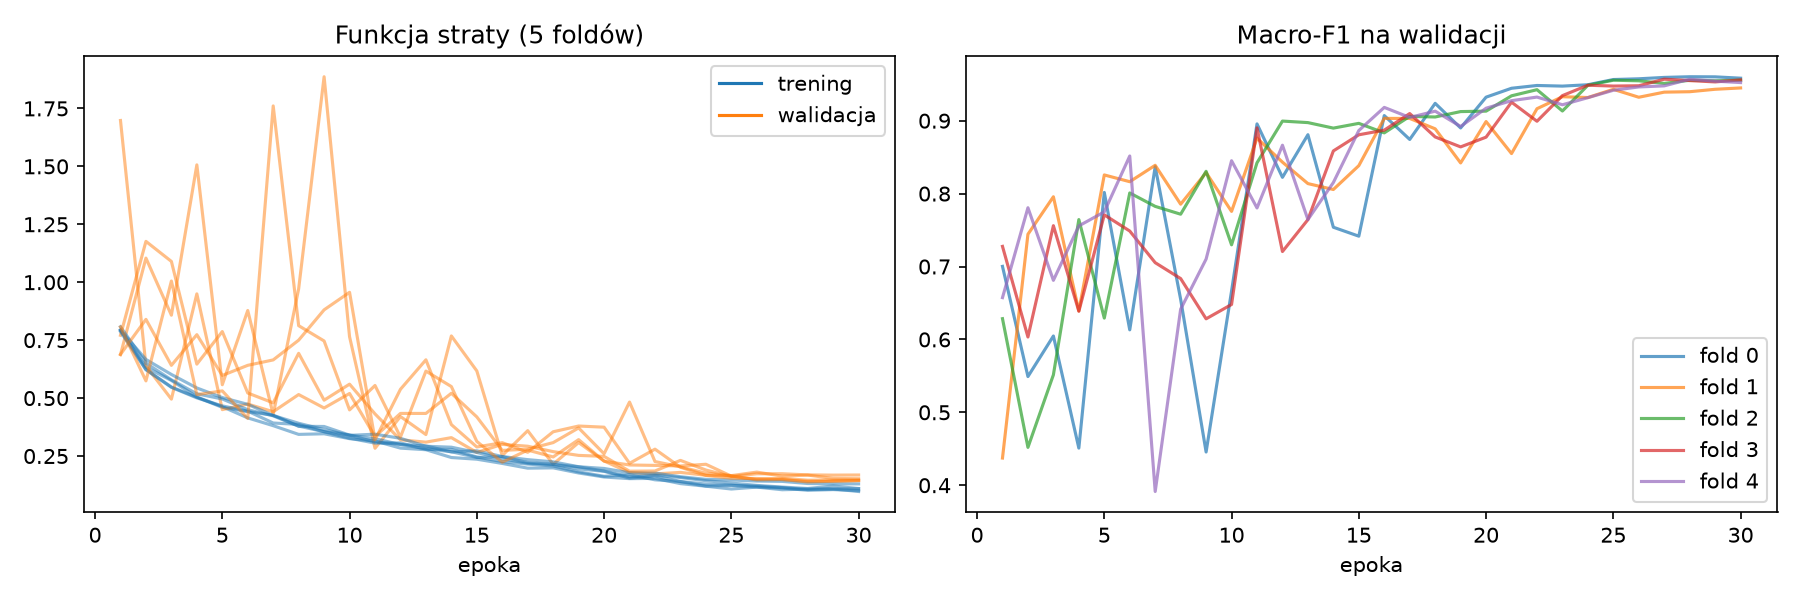
\includegraphics[width=\linewidth]{cv_cnn_krzywe.png}
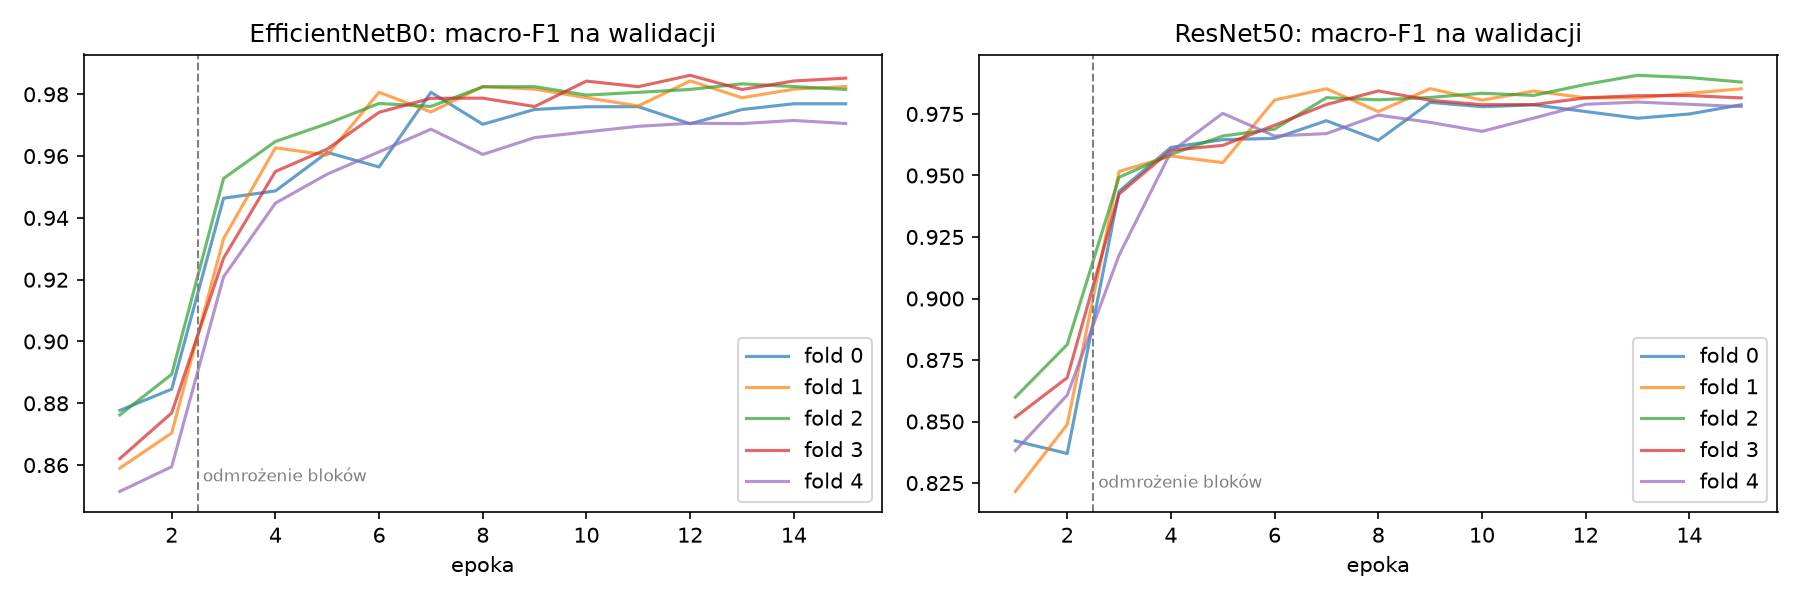
\includegraphics[width=\linewidth]{cv_transfer_krzywe.png}
\caption{Krzywe uczenia w 5 foldach: CNN od zera (góra) oraz macro-F1 na walidacji dla
EfficientNetB0 i ResNet50 (dół). Linia przerywana -- odmrożenie bloków szkieletu.}
\label{fig:krzywe}
\end{figure}

\subsection*{Ewaluacja}
Metryki (\texttt{src/metrics.py}) liczone w układzie ,,klasa kontra reszta'':
\begin{itemize}
\item \textbf{czułość} (recall) $= TP/(TP+FN)$ -- jaki odsetek obrazów danej klasy model wykrył,
\item \textbf{swoistość} $= TN/(TN+FP)$ -- jaki odsetek obrazów innych klas model poprawnie
  do tej klasy nie przypisał,
\item \textbf{precyzja} $= TP/(TP+FP)$, \textbf{F1} (średnia harmoniczna precyzji i czułości),
  \textbf{macro-F1} (średnia F1 z czterech klas -- metryka główna),
\item \textbf{ROC AUC} dla każdej klasy i jego średnia (macro AUC),
\item \textbf{95\,\% przedziały ufności} metodą bootstrap (1000 losowań testu ze zwracaniem,
  percentyle 2,5 i 97,5),
\item \textbf{ECE} (błąd kalibracji): ważona średnia różnica między pewnością a trafnością
  w 10 przedziałach pewności.
\end{itemize}
Z klinicznego punktu widzenia (wykład 4) najważniejsza jest czułość dla klas z guzem
(przeoczenie guza opóźnia leczenie) oraz swoistość klasy \texttt{notumor}, czyli to, jak rzadko
obraz z guzem dostaje wynik ,,brak guza'' (fałszywe uspokojenie). Pomyłka glejak$\leftrightarrow$oponiak
też ma znaczenie, bo te guzy leczy się inaczej (oponiak zwykle chirurgicznie i z dobrym
rokowaniem, glejak wymaga pilnej diagnostyki i często leczenia onkologicznego), ale zawsze
prowadzi do dalszej diagnostyki, więc jest mniej groźna niż przeoczenie guza.

\paragraph{Wyniki walidacji krzyżowej} (tab.~\ref{tab:cv}). Oba modele z transferem wiedzy
są wyraźnie lepsze od CNN od zera (macro-F1 \cvFEff{} i \cvFRes{} wobec \cvFCnn{}). ResNet50
ma najwyższą średnią, ale różnica względem EfficientNetB0 jest mniejsza niż odchylenie
między foldami, więc oba modele są praktycznie równorzędne. EfficientNetB0 jest przy tym
ok.~6 razy mniejszy i 2 razy szybszy (\cvSecEff{} wobec \cvSecRes{} s na epokę).
Według przyjętej reguły (najwyższa średnia w CV) do strojenia wybrano ResNet50.

\begin{table}[H]
\centering
\small
\caption{Walidacja krzyżowa (5 foldów, średnia $\pm$ odchylenie standardowe). ,,najl. ep.'' --
mediana najlepszej epoki / liczba epok.}
\label{tab:cv}
\resizebox{\linewidth}{!}{\tabela{cv}}
\end{table}

\begin{figure}[H]
\centering
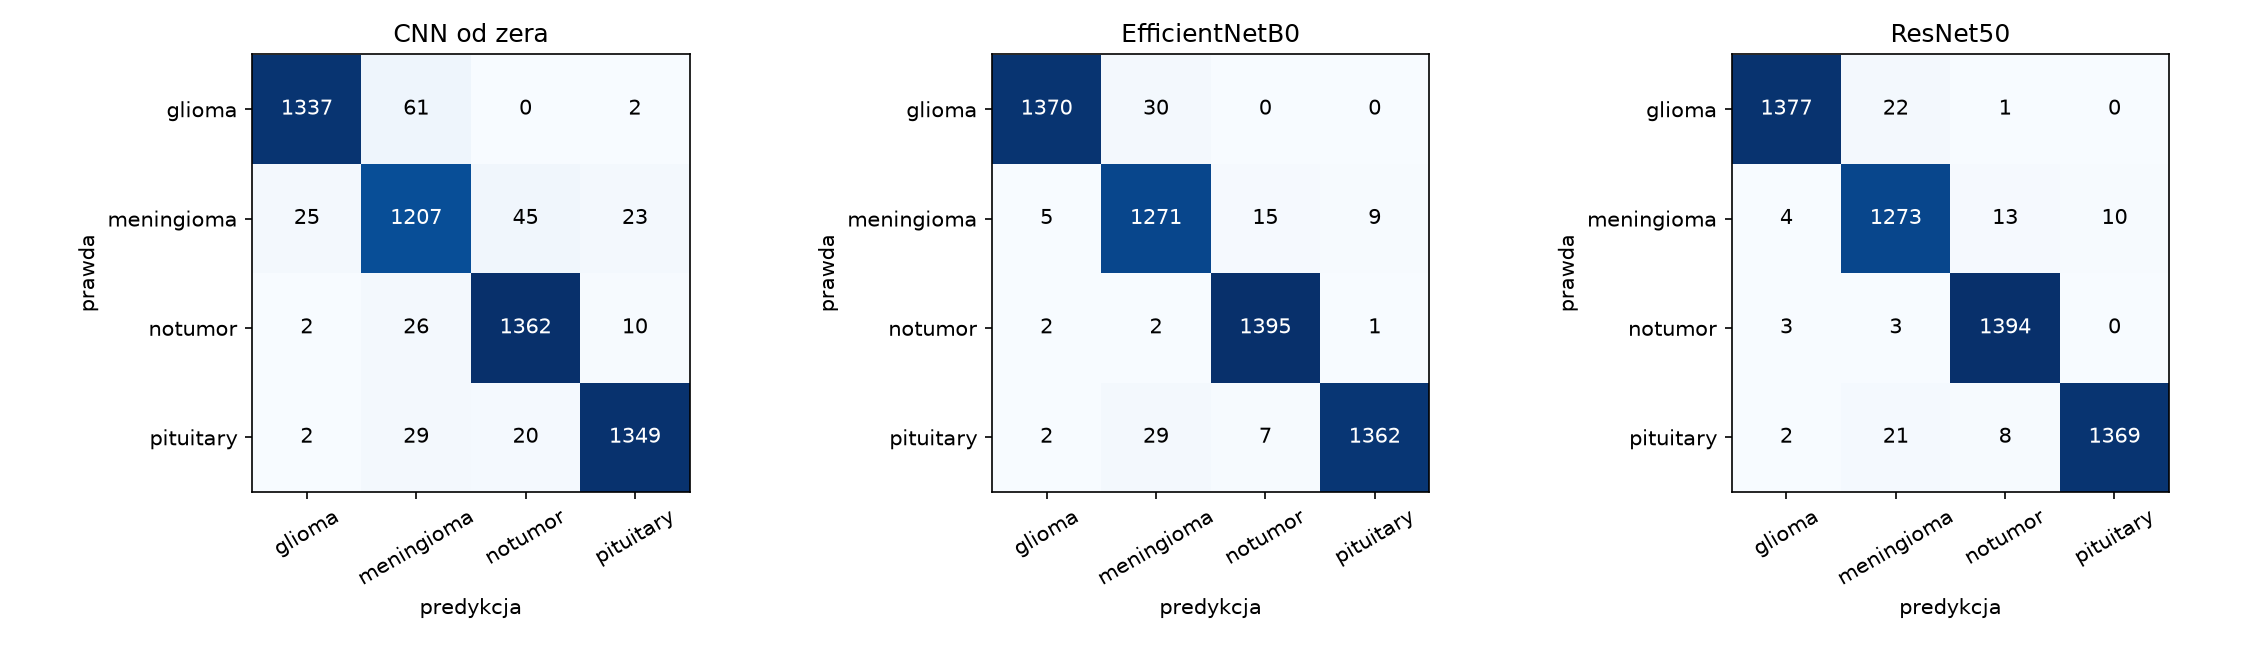
\includegraphics[width=\linewidth]{cv_macierze_oof.png}
\caption{Macierze pomyłek z predykcji out-of-fold (każdy obraz treningowy oceniony przez model,
który go nie widział).}
\label{fig:oof}
\end{figure}

\paragraph{Wyniki na zbiorze testowym} (tab.~\ref{tab:test}).
Zbiór testowy został użyty jeden raz, dla czterech modeli końcowych. Najlepszy model,
ResNet50 po strojeniu, osiąga na oryginalnym teście accuracy \accTestResTuned{}
(95\,\% CI \accCiTestResTuned{}) i macro-F1 \fTestResTuned{}. Na teście oczyszczonym
z duplikatów wyniki są wyraźnie niższe: accuracy \accDedupResTuned{} (\accCiDedupResTuned{})
i macro-F1 \fDedupResTuned{} (\fCiDedupResTuned{}). Taki sam spadek widać dla wszystkich
modeli. Część oryginalnego testu to kopie obrazów treningowych, które model ,,pamięta''.
Dlatego za miarodajny uważamy wynik na \texttt{test\_dedup}, a wynik na oryginalnym teście
podajemy tylko dla porównania z literaturą. Kolejność modeli jest taka sama jak w CV
(CNN wyraźnie najsłabsza), ale przedziały ufności EfficientNetB0 i obu wersji ResNet50
w dużej mierze się pokrywają. Strojenie nie dało więc istotnej statystycznie poprawy.

Wyniki na teście są niższe niż w walidacji krzyżowej (macro-F1 \cvFResTuned{} po strojeniu). Wyjaśnia to
analiza błędów (rozdz.~\ref{sec:bledy}): w teście są glejaki z innego źródła danych,
których w treningu nie było. Wartości per klasa (tab.~\ref{tab:klasy-test} i
\ref{tab:klasy-dedup}) pokazują, że wszystkie błędy dotyczą praktycznie jednej klasy:
\begin{itemize}
\item czułość dla glejaka wynosi tylko \sensDedupGlioma{} (\sensCiDedupGlioma{}) na \texttt{test\_dedup},
  przy swoistości \specDedupGlioma{} -- model nigdy nie nazywa glejakiem czegoś innego,
  ale co piąty glejak umyka,
\item czułość dla oponiaka, guza przysadki i klasy \texttt{notumor} jest bliska 1,
\item swoistość klasy \texttt{notumor} to \specDedupNotumor{} (\specCiDedupNotumor{}): część
  obrazów z guzem (glejaków) model uznaje za obraz bez guza. Klinicznie to najgroźniejszy błąd
  (fałszywe uspokojenie),
\item AUC dla wszystkich klas jest wysokie (glejak \aucDedupGlioma{}, pozostałe $\geq$ 0,98),
  co oznacza, że prawdopodobieństwa porządkują obrazy dość dobrze. Problem leży w progu
  decyzyjnym i w pewności modelu na obrazach spoza znanej dystrybucji.
\end{itemize}
Kalibracja (rys.~\ref{fig:kal}) jest przyzwoita (ECE \eceDedupResTuned{} na \texttt{test\_dedup}),
ale błędy na glejakach mają pewność bliską 1, więc wysoka pewność nie chroni przed pomyłką.
Na małym oczyszczonym teście (tylko \nDedupNotumor{} obrazów \texttt{notumor}) przedziały ufności są
szerokie -- dlatego je raportujemy.


\begin{table}[H]
\centering
\small
\caption{Wyniki na teście oryginalnym i oczyszczonym (w nawiasach 95\,\% przedziały ufności z bootstrapu).}
\label{tab:test}
\resizebox{\linewidth}{!}{\tabela{test}}
\end{table}

\begin{table}[H]
\centering
\small
\caption{Metryki per klasa najlepszego modelu (ResNet50 po strojeniu) na teście oryginalnym.}
\label{tab:klasy-test}
\resizebox{\linewidth}{!}{\tabela{klasy_test}}
\end{table}

\begin{table}[H]
\centering
\small
\caption{Metryki per klasa najlepszego modelu na teście oczyszczonym (\texttt{test\_dedup}).}
\label{tab:klasy-dedup}
\resizebox{\linewidth}{!}{\tabela{klasy_dedup}}
\end{table}

\begin{figure}[H]
\centering
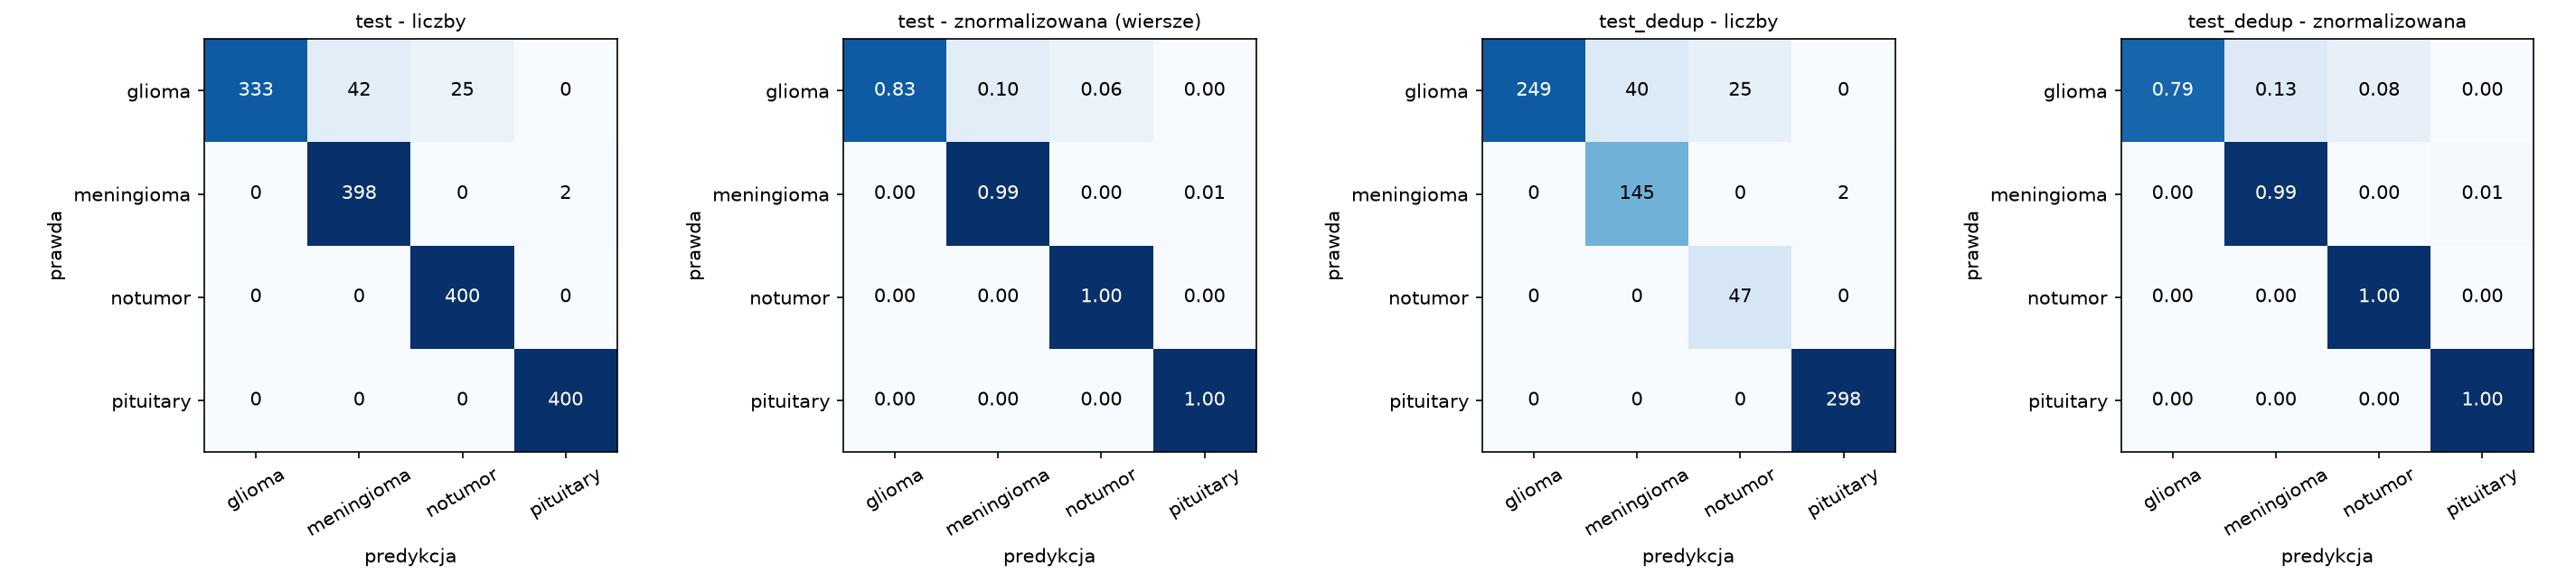
\includegraphics[width=\linewidth]{test_macierze.png}
\caption{Macierze pomyłek najlepszego modelu: test oryginalny i oczyszczony (liczby i wartości
znormalizowane wierszami, czyli czułość na przekątnej).}
\label{fig:cm}
\end{figure}

\begin{figure}[H]
\centering
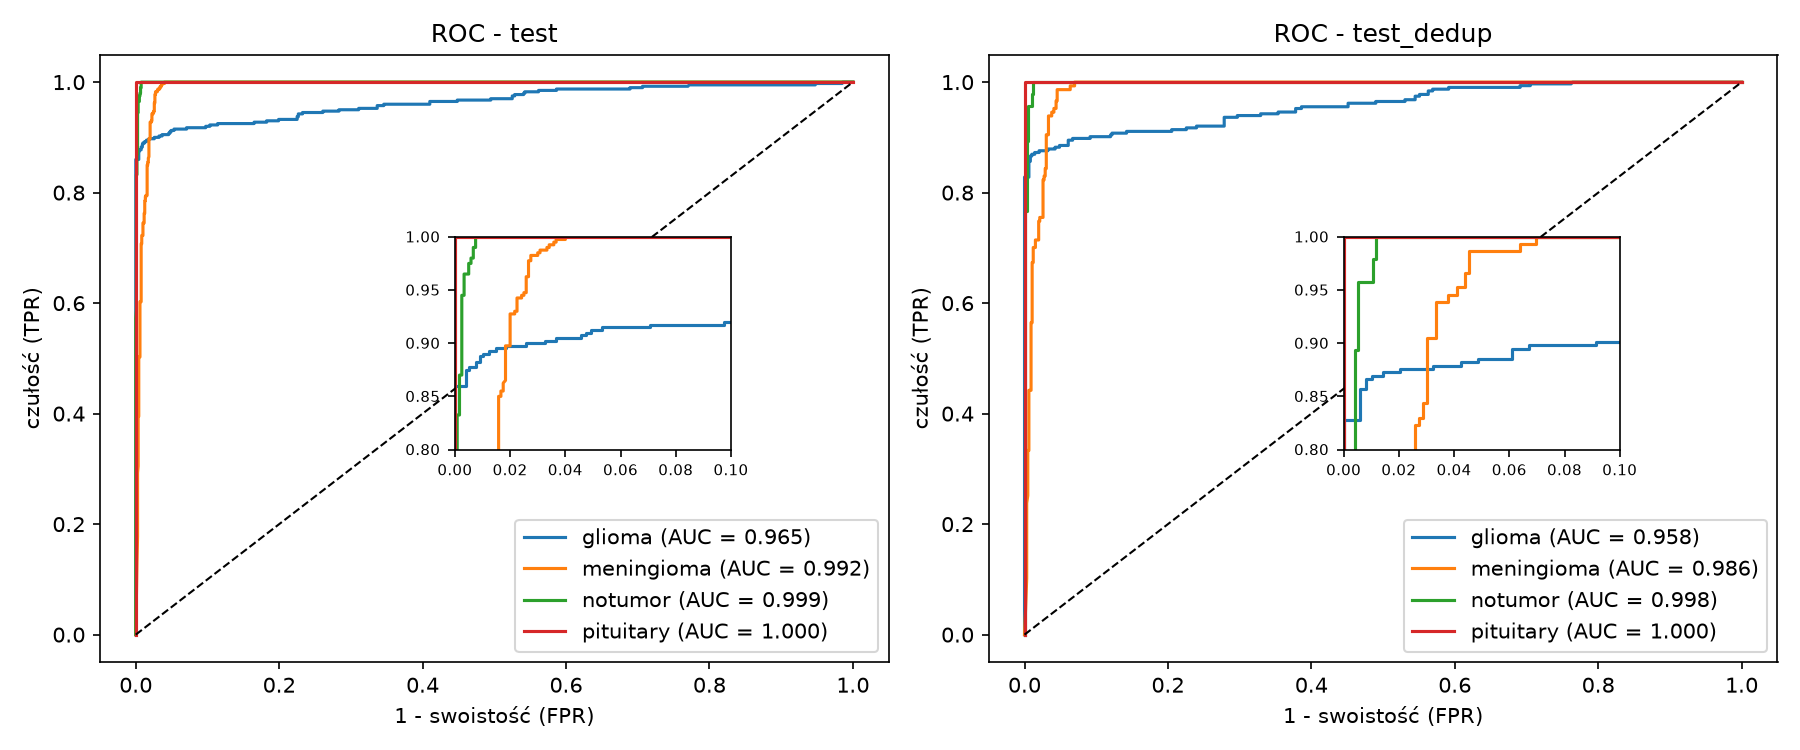
\includegraphics[width=\linewidth]{test_roc.png}
\caption{Krzywe ROC (klasa kontra reszta) najlepszego modelu; wstawki -- powiększenie lewego górnego rogu.}
\label{fig:roc}
\end{figure}

\begin{figure}[H]
\centering
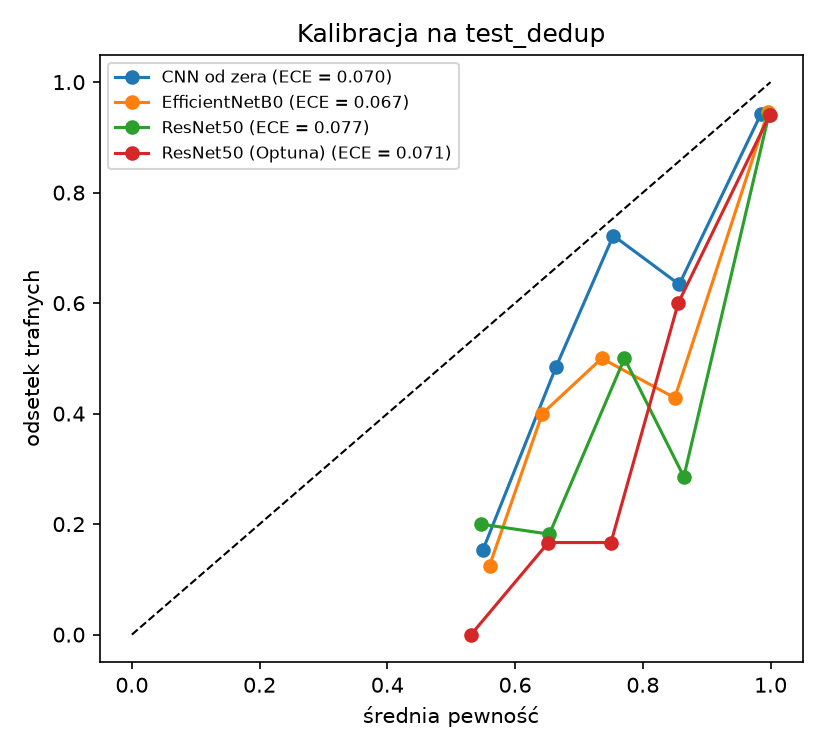
\includegraphics[width=0.55\linewidth]{test_kalibracja.png}
\caption{Wykres niezawodności (kalibracja) na teście oczyszczonym.}
\label{fig:kal}
\end{figure}

\subsection*{Dobór hiperparametrów}
Hiperparametry najlepszej architektury (ResNet50) dobrano biblioteką \textbf{Optuna}
(\texttt{src/tune.py}, notatnik \texttt{04\_tuning\_optuna.ipynb}). Jest to optymalizacja
bayesowska, a nie przeszukiwanie siatki ani losowe. Próbnik TPE (Tree-structured Parzen
Estimator) dzieli dotychczasowe próby na lepsze i gorsze, modeluje rozkład hiperparametrów
w obu grupach i proponuje konfiguracje, dla których stosunek tych rozkładów jest największy.
Słabe próby przerywa MedianPruner: po każdym foldzie porównuje średni wynik próby z medianą
wcześniejszych prób na tym samym etapie (idea Successive Halving z wykładu).

Przestrzeń poszukiwań: LR głowicy $10^{-4}$--$3\cdot10^{-3}$ (skala logarytmiczna), weight decay
$10^{-6}$--$10^{-2}$ (log.), dropout 0--0,5, batch size \{16, 32, 64\}, liczba odmrożonych
bloków szkieletu 1--\nBlocks{}. Funkcja celu to średnie macro-F1 na foldach walidacyjnych 0--2
(10 epok na próbę). Zbiór testowy nie był używany. Badanie liczy \nTrials{} prób
(\nTrialsComplete{} zakończonych, \nTrialsPruned{} przyciętych). Dodatkowo jedna próba została
przerwana przez wyłączenie komputera. Optuna zapisuje próby w bazie SQLite, więc strojenie wznowiono
i dokończono do \nTrials{} prób.

Najlepsza konfiguracja: LR $\optLr$, weight decay $\optWd$, dropout \optDropout{}, batch size
\optBatch{}, \optUnfreeze{} odmrożone bloki. Najważniejszym hiperparametrem okazał się LR
(ważność fANOVA \impLr{}), potem dropout (\impDropout{}) i weight decay (\impWd{}).

\begin{figure}[H]
\centering
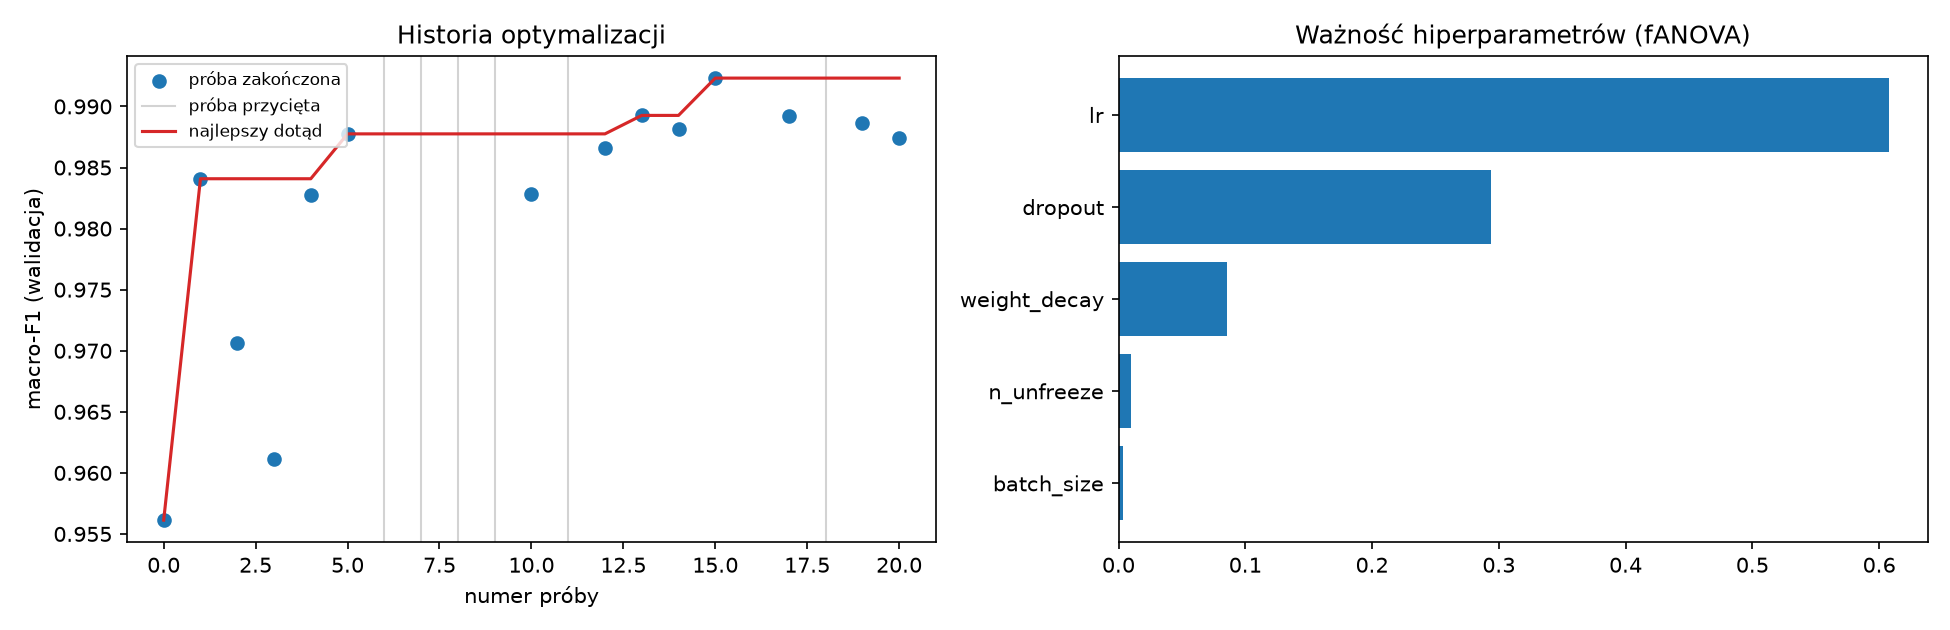
\includegraphics[width=\linewidth]{optuna.png}
\caption{Historia optymalizacji (szare linie -- próby przycięte) i ważność hiperparametrów.}
\label{fig:optuna}
\end{figure}

\paragraph{Ryzyko przeoptymalizowania na walidacji.} Najlepsza próba osiągnęła na walidacji
macro-F1 \optBest{}, ale ta liczba jest zawyżona. Wybieramy maksimum z wielu prób liczonych na
tych samych foldach, więc część przewagi to przypadek (wykład~4). W pełnej 5-krotnej walidacji
parametry po strojeniu dały \cvFResTuned{} $\pm$ \cvFsdResTuned{} wobec \cvFRes{} $\pm$ \cvFsdRes{}
dla parametrów domyślnych. Poprawa jest mniejsza niż odchylenie między foldami, a foldy 0--2
służyły do strojenia. Poprawną metodą byłaby zagnieżdżona walidacja krzyżowa, jednak jest
ok.~5 razy droższa obliczeniowo. Ostatecznym sprawdzianem był test: po strojeniu macro-F1 na
\texttt{test\_dedup} wzrosło z \fDedupRes{} do \fDedupResTuned{}, ale przedziały ufności
się pokrywają.

